%! TEX root = ./talk_slides.tex
\documentclass{beamer}
\usepackage[utf8]{inputenc}
\usepackage{amsmath}
\usepackage{amssymb}
\usepackage{amsfonts}
\usepackage{amstext}
\usepackage{amsthm}
\usepackage{enumerate}
\usepackage{graphicx}
\usepackage{ytableau}
\usepackage{hyperref}
\usepackage{tikz}
\usetikzlibrary{arrows.meta,shapes,positioning,calc,patterns}
\tikzset{cross/.style={cross out, draw=black, minimum size=2*(#1-\pgflinewidth), inner sep=0pt, outer sep=0pt},
%default radius will be 1pt. 
cross/.default={1pt}}

\usepackage[colorinlistoftodos]{todonotes}
\newcommand{\Jen}[1]{\todo[size=\tiny,color=orange!30]{#1
      \\ \hfill --- Jenn}}




\newcommand{\jen}[1]{\textcolor{orange}{#1}}
\newcommand{\jennifer}[1]{\textcolor{orange}{#1}}


\renewcommand{\thesubsection}{\thesection.\alph{subsection}}
\setlength{\parindent}{0pt}

\setbeamertemplate{footline}[page number]{}
\beamertemplatenavigationsymbolsempty

\newcommand{\comment}[1]{}
\newcommand{\set}[1]{\{ #1 \}}


% \newtheorem{corollary}[theorem]{Corollary}
% \newtheorem{lemma}[theorem]{Lemma}
%\newtheorem{proposition}[theorem]{Proposition}
% \theoremstyle{definition}
% \newtheorem{definition}[theorem]{Definition}
% \newtheorem{example}[theorem]{Example}
% \newtheorem{question}[theorem]{Question}
% \theoremstyle{remark}
% \newtheorem{remark}[theorem]{Remark}
% %----------------------------------------------------------
\title{The Area of $(sn,n)$ Dyck Paths}
\author{Evan Conway \and James Harbour \and Henghui Li \and Luke Moyar}

\begin{document}
\frame{\titlepage}

\begin{frame}{Contents}
\tableofcontents
\end{frame}

\section{Motivation}
\subsection{$(n, n)$ Paths}

\begin{frame}{Dyck Paths of Type $(n,n)$}
\begin{definition}
A lattice path from $(0, 0)$ to $(n, n)$ consisting of only the steps $(1, 0)$ and $(0, 1)$ such that the path never goes above the diagonal.
\end{definition}

\begin{example}
Two paths of type $(4,4)$:
\begin{figure}
    \centering
    \includegraphics[width=0.85\linewidth, angle = 180]{Dyck_Examples_1.png}
\end{figure}
\end{example}
\end{frame}

\begin{frame}{The Area of a Dyck Path}
\begin{definition}
The number of complete squares between the path and the diagonal. 
\end{definition}
\begin{example}
All Dyck paths of length 6 and their corresponding areas:
\begin{figure}
    \centering
    \includegraphics[width=0.75\linewidth]{path_and_og_area.png}
\end{figure}
\end{example}
\end{frame}

\begin{frame}{The Area of a Dyck Path}
We include partial boxes as well (this can be easily converted over)

\begin{example}
All Dyck paths of length 6 and their corresponding "full" areas:
\begin{figure}
    \centering
    \includegraphics[width=0.75\linewidth]{path_and_new_area.png}
\end{figure}
\end{example}
\end{frame}

\begin{frame}{The Total Area Statistic}
    \uncover<1->{\textbf{Question}: What is the total area of all Dyck paths of type $(n,n)$?}
    \newline

    \uncover<2->{\begin{theorem}
    The total area of all Dyck paths of type $(n,n)$ is
      \[
        A_{n} = \frac{1}{2} \left(4^{n}-\binom{2n+1}{n}\right) 
      \]
    \end{theorem}}

    
    \uncover<3->{How do we find this? Well, we could try finding a recursive relation...}
\end{frame}

\begin{frame}{Computing the Total Area Statistic: Part 1}
    How to find a recursive relation for area? Split by first touch point!

    \begin{figure}
        \centering
        \includegraphics[width=1\linewidth]{split_dyck.png}
    \end{figure}

    There are \textbf{no} touch points before the first!
\end{frame}

\begin{frame}{Computing the Total Area Statistic: Part 2}
    Breaking down area: (arcs are paths that are \textbf{not determined})

    \begin{figure}
        \centering
        \includegraphics[width=0.75\linewidth]{Summing Dyck Area.png}
    \end{figure}

    Areas:
    \begin{itemize}
        \item $(i)$: trapezoid area that \textbf{must} be included
        \item $(ii)$ and $(iii)$: area of smaller Dyck paths
    \end{itemize}
\end{frame}

\begin{frame}{Computing the Total Area Statistic: Part 3}
    Summing the area of the every path amounts to the area of each area i, ii, and iii.
    \begin{enumerate}[i]
        \item The area of a 
    \end{enumerate}
    
\end{frame}

\begin{frame}{Average Area for Type $(n,n)$}
    \textbf{Question}: we have formulas for the total area and total number of paths — what is the average area?
\end{frame}

\begin{frame}{Average Area for Type $(n,n)$}

Exact average area is messy, but with asymptotics we can simplify!

\begin{theorem}
As a result of Stirling's approximation, it holds that
\begin{align*}
\frac{A_n}{c_n} &= \frac{1}{2}\cdot\frac{n+1}{\binom{2n}{n}}( \left(4^{n} - \binom{2n+1}{n}\right))
\\ &\sim \frac{1}{2} \left({\frac{(n+1)4^{n}}{\frac{2^{2n}}{\sqrt{\pi n}}} - (2n+1)}\right)
\\ &\sim \frac{\sqrt{\pi}}{2} n^{3/2} \asymp n^{3/2}
\end{align*}
\end{theorem}
\end{frame}

\subsection{Generalizing Dyck Paths}
\begin{frame}{What Next?}
    \uncover<1->{\textbf{Question}: can we generalize Dyck paths and also get nice facts about their area?}
    \newline
    
    \uncover<2->{Generalizations of Dyck paths:
    
    \begin{itemize}
        \item Higher-Dimensional Paths
        \item General $(m,n)$ Paths
        \item $(m,n)$ Paths when $m, n$ coprime
        \item $(sn,n)$ Paths
    \end{itemize}}
\end{frame}

\begin{frame}{$(sn,n)$ Paths - A Workable Case}

Benefits:
\begin{itemize}
    \item Can use same area (unlike higher dimensions)
    \item Has touch points (unlike $m, n$ coprime)
    \item Might be able to generalize previous recurrence
\end{itemize}

\begin{example} A path in $k = 2, n = 3$:
\begin{center}
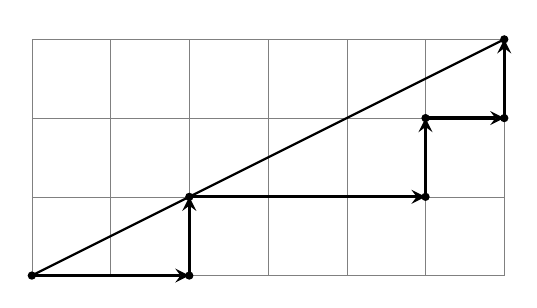
\begin{tikzpicture}[scale=1, every node/.style={scale=1}]
    % Define dimensions
    \def\n{3}
    \def\k{2}
    
    % Draw grid
    \draw[gray, very thin] (0,0) grid (\n*\k,\n);
    
    % Draw diagonal
    \draw[black, thick] (0,0) -- (\n*\k,\n) node[anchor=south west] [xshift=-1.5cm,yshift=-0.1cm] {};

    \coordinate (A) at (0,0);
    \coordinate (B) at (2,0);
    \coordinate (C) at (2,1);
    \coordinate (D) at (5,1);
    \coordinate (E) at (5,2);
    \coordinate (F) at (6,2);
    \coordinate (G) at (6,3);

    %Draw lines between adjacent points
    \foreach [remember=\point as \previouspoint (initially A)] \point in {B,C,D,E,F,G} {
        \draw[very thick, -stealth] (\previouspoint) -- (\point);
    }
    
    %Draw points
    \foreach \point in {A, B, C, D, E, F, G}
        \fill [black] (\point) circle (1.5pt);
\end{tikzpicture}
\end{center}
\end{example}
\end{frame}

\section{Working with Paths of Type $(sn,n)$}
\begin{frame}{Counting Paths of Type $(sn,n)$: Overall Strategy}
    \uncover<1->{How can we adapt our strategy from the type $(n,n)$ case?}
    \newline

    \pause

    \begin{enumerate}[<+->]
        \item Instead of only talking about touchpoints on the "center" line ($x = sy$), we add extra lines $x = sy + i$ for $1 \leq i < s$ and talk about the touch points on those as well
        \item We can characterize paths by their last touch points on our original line and our new lines. We can then use these touch points to find a recursive relation for our path counts.
    \end{enumerate}
\end{frame}

\begin{frame}{Counting Paths of Type $(sn,n)$: Overall Strategy}
    \begin{example} A path in $k = 2, n = 3$, with our new lines added and their last touch points marked:
    \begin{center}
    \begin{tikzpicture}[scale=1, every node/.style={scale=1}]
        % Define dimensions
        \def\n{3}
        \def\k{2}
        
        % Draw grid
        \draw[gray, very thin] (0,0) grid (\n*\k,\n);
        
        % Draw diagonal
        \draw[black, thick] (0,0) -- (\n*\k,\n) node[anchor=south west] [xshift=-1.5cm,yshift=-0.1cm] {};
        \draw[black, dashed] (1,0) -- (\n*\k,\n-1/\k) node[anchor=south west] [xshift=-1.5cm,yshift=-0.1cm] {};
    
        \coordinate (A) at (0,0);
        \coordinate (B) at (2,0);
        \coordinate (C) at (2,1);
        \coordinate (D) at (5,1);
        \coordinate (E) at (5,2);
        \coordinate (F) at (6,2);
        \coordinate (G) at (6,3);
    
        %Draw lines between adjacent points
        \foreach [remember=\point as \previouspoint (initially A)] \point in {B,C,D,E,F,G} {
            \draw[very thick, -stealth] (\previouspoint) -- (\point);
        }
        
        %Draw points
        \foreach \point in {A, B, C, D, E, F, G}
            \fill [black] (\point) circle (1.5pt);

        \foreach \point in {C,E}
            \fill [black] (\point) cross (3pt);
    \end{tikzpicture}
    \end{center}
    \end{example}
\end{frame}

\section{Counting the Total Area Statistic on $(sn,n)$ Paths}
\begin{frame}{Summing Area: Strategy}
    \begin{enumerate}
        \item Adapt the method used to \textit{count} $(sn,n)$ paths to find a recursive relation for the area
        \item Isolate the area in the recursive relation
        \item Solve for a closed formula
    \end{enumerate}
\end{frame}

\begin{frame}{Summing Area: Overall Formula}
    \begin{align*}
    & A_{n+1} = \sum_{\substack{0\leq y_{0}\leq \cdots\leq y_{s-1}\leq n\\y_{s}=n}} \sum_{\substack{P\in \mathcal{D}_{n+1}^{s}\\\text{of type }y_{0},\ldots, y_{s-1}}} \text{area}(P) \\
    &= \sum_{\substack{0\leq y_{0}\leq \cdots\leq y_{s-1}\leq n\\y_{s}=n}} \sum_{\substack{P\in \mathcal{D}_{n+1}^{s}\\\text{of type }y_{0},\ldots, y_{s-1}}} \left( \sum_{k=1}^{s}I_{l} + \sum_{l=0}^{s}\text{area}(P_{l}) \right) \\
    &= \sum_{\substack{0\leq y_{0}\leq \cdots\leq y_{s-1}\leq n\\y_{s}=n}} \sum_{\substack{P\in \mathcal{D}_{n+1}^{s}\\\text{of type }y_{0},\ldots, y_{s-1}}} \bigg( \sum_{l=1}^{s}\frac{1}{s}(l-\frac{1}{2}) +l(y_{l}-y_{l-1}) \\ & + \sum_{l=0}^{s}\text{area}(P_{l}) \bigg)
\end{align*}
\end{frame}

\begin{frame}{Non-Recursive Breakdown}
Note: need to insert an image here to show what the polygons look like.
\end{frame}

\begin{frame}{Non-Recursive Breakdown}
We wish to simplify the following, which will let us find the non-recursive part of our area breakdown:

\begin{align*}
  \sum_{\substack{0\leq y_{0}\leq \cdots\leq y_{s-1}\leq n\\y_{s}=n}} \sum_{\substack{P\in \mathcal{D}_{n+1}^{s}\\ \text{of type }y_{0},\ldots, y_{s-1}}} \left( \sum_{l=1}^{s}\frac{1}{s}(l-\frac{1}{2}) +l(y_{l}-y_{l-1}) \right).
\end{align*}

\end{frame}

\section{Detailed Expansion}
\begin{frame}
\frametitle{Detailed Expansion: Part 1}

We begin by breaking down the following sum into understandable parts:
\[
  \sum_{l=1}^{s}\frac{1}{s}\left(l-\frac{1}{2}\right) = \frac{1}{s}\cdot \frac{s(s+1)}{2}-\frac{1}{s}\cdot\frac{s}{2} = \frac{s}{2}.
\]
This computation serves as a foundation for further analysis in our problem.
\end{frame}

\begin{frame}
\frametitle{Detailed Expansion: Part 1}
Now we expand 
\begin{align*}
  & \sum_{\substack{0\leq y_{0}\leq \cdots\leq y_{s-1}\leq n\\y_{s}=n}} \sum_{\substack{P\in \mathcal{D}_{n+1}^{s}\\\text{of type }y_{0},\ldots, y_{s-1}}} \frac{s}{2} \\
  & = \frac{s}{2} \sum_{\substack{0\leq y_{0}\leq \cdots\leq y_{s-1}\leq n\\y_{s}=n}}  F_{s+1}(y_{0}) \cdot \prod_{1\leq i \leq s} F_{s+1}(y_{i}-y_{i-1}) \\
  & = \frac{s}{2} \sum_{k=0}^{n}F_{s+1}(k)[F(z)^{s}]_{n-k} = \frac{s}{2} [F(z)^{s+1}]_{n} 
\end{align*}
\end{frame}

\begin{frame}
\frametitle{Detailed Expansion: Part 2}
Next, we simplify the second part of our sum:
\begin{align*}
  & \sum_{\substack{0\leq y_{0}\leq \cdots\leq y_{s-1}\leq n\\y_{s}=n}} \sum_{\substack{P\in \mathcal{D}_{n+1}^{s}\\ \text{of type }y_{0},\ldots, y_{s-1}}} \sum_{l=1}^{s} l(y_{l}-y_{l-1}) \\
  &= \sum_{l=1}^{s}l\sum_{k=0}^{n}F_{s+1}(k) \sum_{d_{1}+\cdots+d_{s}=n-k}  d_{l}\cdot  \prod_{1\leq i \leq s} F_{s+1}(d_{i})\\
  & = \sum_{l=1}^{s}l \cdot[zF^{\prime}(z)F(z)^{s}]_{n} = {s+1 \choose 2}[zF^{\prime}(z)F(z)^{s}]_{n}
\end{align*}
\end{frame}

\begin{frame}
\frametitle{Non-Recursive Formula}
Combining these two parts, we obtain this formula for the non-recursive part of the area:

\begin{align*}
  \frac{s}{2} [F(z)^{s+1}]_{n} + {s+1 \choose 2}[zF^{\prime}(z)F(z)^{s}]_{n}
\end{align*}
\end{frame}

\begin{frame}{Recursive Breakdown}
Note: need to insert an image here to show what the recursive sections look like.
\end{frame}

\begin{frame}{Recursive Breakdown}
We wish to simplify the following, which will let us find the recursive part of our area breakdown:

\begin{align*}
  \sum_{\substack{0\leq y_{0}\leq \cdots\leq y_{s-1}\leq n\\y_{s}=n}} &\sum_{\substack{P\in \mathcal{D}_{n+1}^{s}\\\text{of type }y_{0},\ldots, y_{s-1}}}  \sum_{l=0}^{s} \text{area}(P_{l})
\end{align*}
\end{frame}

\begin{frame}{Detailed Expansion}
We can split up our starting sum into two parts:

\begin{align*}
  & \sum_{\substack{0\leq y_{0}\leq \cdots\leq y_{s-1}\leq n\\y_{s}=n}} \sum_{\substack{P\in \mathcal{D}_{n+1}^{s}\\\text{of type }y_{0},\ldots, y_{s-1}}}  \sum_{l=0}^{s} \text{area}(P_{l}) \\
  & = \sum_{\substack{0\leq y_{0}\leq \cdots\leq y_{s-1}\leq n\\y_{s}=n}} \sum_{\substack{P\in \mathcal{D}_{n+1}^{s}\\\text{of type }y_{0},\ldots, y_{s-1}}} \text{area}(P_{0}) \\ 
  & +\sum_{l=1}^{s} \sum_{\substack{0\leq y_{0}\leq \cdots\leq y_{s-1}\leq n\\y_{s}=n}} \sum_{\substack{P\in \mathcal{D}_{n+1}^{s}\\\text{of type }y_{0},\ldots, y_{s-1}}} \text{area}(P_{l})
\end{align*}
\end{frame}

\begin{frame}{Detailed Expansion, Part 1}
We can simplify our first sum:

\begin{align*}
  & \sum_{\substack{0\leq y_{0}\leq \cdots\leq y_{s-1}\leq n\\y_{s}=n}} \sum_{\substack{P\in \mathcal{D}_{n+1}^{s}\\\text{of type }y_{0},\ldots, y_{s-1}}} \text{area}(P_{0}) \\
  & = \sum_{k=0}^{n}\sum_{d_{1}+\cdots+d_{s}=n-k} \sum_{\gamma\in \mathcal{D}_{k}^{s}}  \text{area}(\gamma)\cdot \prod_{1\leq i\leq s}F_{s+1}(d_{i}) \\
  & = \sum_{k=0}^{n}A_{k}[F(z)^{s}]_{n-k} = [A(z)F(z)^{s}]_{n}
\end{align*}
\end{frame}

\begin{frame}{Detailed Expansion, Part 2}
We can also simplify our second sum:

\begin{align*}
  & \sum_{l=1}^{s}\sum_{\substack{0\leq y_{0}\leq \cdots\leq y_{s-1}\leq n\\y_{s}=n}} \sum_{\substack{P\in \mathcal{D}_{n+1}^{s}\\\text{of type }y_{0},\ldots, y_{s-1}}} \text{area}(P_{l}) \\
  &= \sum_{l=1}^{s} \sum_{k=0}^{n}F_{s+1}(k)\sum_{r=0}^{n-k}A_{r}\sum_{k_{1}+\cdots+k_{s-1} = n-k-r}  F_{s+1}(k_{1})\cdots F_{s+1}(k_{s-1}) \\
  & = \sum_{l=1}^{s} \sum_{k=0}^{n}[F(z)]_{k}\cdot[A(z)F(z)^{s-1}]_{n-k} = s[A(z)F(z)^{s}]_{n}
\end{align*}
\end{frame}

\begin{frame}
\frametitle{Recursive Formula}
Combining these two parts, we obtain this formula for the recursive part of the area:

\begin{align*}
  & [A(z)F(z)^{s}]_{n} + s[A(z)F(z)^{s}]_{n} \\
  & = (s+1) [A(z)F(z)^{s}]_{n}
\end{align*}
\end{frame}

\begin{frame}
\frametitle{Combined Formula}
Combine recursive and non-recursive:

\begin{align*}
  A_{n+1} = \frac{s}{2} [F(z)^{s+1}]_{n} + {s+1 \choose 2}[zF^{\prime}(z)F(z)^{s}]_{n} + (s+1) [A(z)F(z)^{s}]_{n}
\end{align*}

Transforming to isolate area:

\begin{align*}
    A(z) = \frac{s}{2} zF'(z) + {s+1 \choose 2} \cdot \frac{1}{F(z)} \cdot (zF'(z))^2
\end{align*}

\end{frame}

\begin{frame}{Area Equation Transformation}

Take functional equation:

\begin{align*}
    A(z) = \frac{s}{2} zF'(z) + {s+1 \choose 2} \cdot \frac{1}{F(z)} \cdot (zF'(z))^2
\end{align*}

Plug in and solve for final area formula:
\begin{center}
    $A_n = \frac{s}{2} {(s+1)n \choose n-1} + {s+1 \choose 2} [\sum_{k=0}^{n} {(s+1)k \choose k-1} {(s+1)(n-k) \choose n-k-1}] - {s+1 \choose 2} \sum_{r=0}^{n-1} \frac{1}{n-r} {(s+1)(n-r)-2 \choose n-r-1} \sum_{k=0}^{r} {(s+1)k \choose k-1} {(s+1)(r-k) \choose r-k-1}$
\end{center}
\end{frame}

\begin{frame}{Future Directions}

Note: this needs to be written closer to presentation time since we are actively researching this

\end{frame}

\end{document}
